% Created 2020-04-24 vie 23:03
% Intended LaTeX compiler: pdflatex
\documentclass[11pt,a4paper]{article}
\usepackage[utf8]{inputenc}
\usepackage[T1]{fontenc}
\usepackage{graphicx}
\usepackage{grffile}
\usepackage{longtable}
\usepackage{wrapfig}
\usepackage{rotating}
\usepackage[normalem]{ulem}
\usepackage{amsmath}
\usepackage{textcomp}
\usepackage{amssymb}
\usepackage{capt-of}
\usepackage{hyperref}
\usepackage{tabularx}
\usepackage{lastpage}
\usepackage{enumitem}
\usepackage[english, spanish]{babel}
\usepackage[table,xcdraw]{xcolor}
\usepackage[left=2.00cm, right=2.50cm, top=2.50cm, bottom=2.50cm]{geometry}


\newcommand*{\autor}[1]{\def\authorname{#1}}
\newcommand*{\titulo}[1]{\def\@title{#1}\def\ttitle{#1}}

\renewcommand{\contentsname}{Índice}
\newcommand{\versionActual}{A}
\newcommand{\fechaA}{13/07/2025}
\newcommand{\fechaB}{}
\newcommand{\fechaC}{}

\newcommand{\docCode}{\normalsize RETRO\_GAME-CU versión \versionActual}

\usepackage{ifthen}
\newcommand{\fechaActual}{%
  \ifthenelse{\equal{\versionActual}{A}}{\fechaA}{%
    \ifthenelse{\equal{\versionActual}{B}}{\fechaB}{%
      \ifthenelse{\equal{\versionActual}{C}}{\fechaC}{
        N/A
      }}}}

\titulo{Videojuego portátil inspirado en consolas retro} 
\autor{Lic. Jezabel Danon}

\usepackage{fancyhdr}
\fancyhf{} % clear all header and footers
\pagestyle{fancy}
\lhead{
\includegraphics[width=3.5cm]{../Figuras/logoFIUBA.pdf}}
\chead{}
\rhead{\normalsize \textrm{ \textbf{\@title} \\ Especificación de casos de uso\\ \docCode}}
\setlength{\footskip}{25pt}
\lfoot{ }
\cfoot{\normalsize Página \thepage \hspace{1px} de \pageref{LastPage}}
\rfoot{}
\setlength{\fboxrule}{4pt} \setlength{\fboxsep}{2ex}
\setlength{\headheight}{42pt}

\renewcommand{\headrulewidth}{1.0pt}
\renewcommand{\footrulewidth}{0.4pt}

\hypersetup{
   colorlinks=true,
  linkcolor=black,      % color para enlaces internos (índice, referencias)
  citecolor=black,      % color para citas (si usás biblatex)
  filecolor=black,      % enlaces a archivos
  urlcolor=blue,        % color para \href y \url
 pdftitle = {\@title},
 pdfauthor = {\authorname},
 pdfkeywords={},
 pdfsubject={},
%  pdfcreator={Emacs 26.2 (Org mode 9.1.9)}, 
 pdflang={es}
}

% ────────── preámbulo: definir ancho utilizable y macro ──────────

\newcommand{\UseCaseTable}[9]{%
\begingroup
\renewcommand{\arraystretch}{1.2}
\noindent 
\rowcolors{3}{white}{white}% sin zebra
\begin{tabularx}{\linewidth}{@{}|>{\raggedright\arraybackslash}p{4cm}|X|@{}}
\hline
\rowcolor[HTML]{0073A0}%
\multicolumn{2}{|c|}{\color{white}\bfseries #1}\\ \hline
\textbf{1.~Nombre} & #1\\ \hline
\textbf{1.1 Breve descripción} & #2\\ \hline
\textbf{1.2 Actor principal} & #3\\ \hline
\textbf{1.3 Disparador} & #4\\ \hline
\multicolumn{2}{|l|}{\textbf{2.~Flujo de eventos}} \\ \hline   % ← aquí el cambio
\quad\textbf{2.1 Flujo básico} & #5\\ \hline
\quad\textbf{2.2 Flujos alternativos} & #6\\ \hline
\textbf{3. Requerimientos especiales} & #7\\ \hline
\textbf{4. Pre-condiciones} & #8\\ \hline
\textbf{5. Post-condiciones} & #9\\ \hline
\end{tabularx}
\endgroup
% \vspace{1em}%
}
% \renewcommand{\thesection}{\arabic{section}.}
% \renewcommand{\thesubsection}{\thesection\arabic{subsection}.}
% \renewcommand{\thesubsubsection}{\thesubsection\arabic{subsubsection}.}

%  COMIENZA EL DOCUMENTO --------------------------------------------------------------------
\begin{document}

% \maketitle
\begin{titlepage}
    \centering

    
\includegraphics[width=.7\textwidth]{../Figuras/logoFIUBA.pdf}\par
    \vspace{1cm}

    
    \vspace{3cm}
    {\Huge \textbf{\ttitle}} \\
    \vspace{2cm}

    {\Large\itshape Especificación de casos de uso\par}
    \vspace{4cm}

    
    
    \flushleft
    {\normalsize Autor:\\}
    {\Large \authorname \ (jezabel.danon@gmail.com)\\}
    \vspace{1.5cm}

    {\scshape\LARGE \fechaActual \par} 
    {\scshape\LARGE Versión \versionActual \par}

    \vfill
    \centering
    \textit{Este documento fue creado durante el curso de Ingeniería de Software entre el 26 de junio de 2025 y el 21 de agosto de 2025.}
\end{titlepage}

\clearpage            % fuerza una nueva página real
\pagestyle{fancy}     % activa encabezado y pie desde esta página

\section*{Historial de cambios}
\pagestyle{fancy}     % activa el estilo fancy para el resto
\begin{table}[ht]
\label{tab:registro}
\centering
\begin{tabularx}{\linewidth}{@{}|c|c|X|c|c|@{}}
\hline
\rowcolor[HTML]{C0C0C0} 
Versión & Fecha & \multicolumn{1}{c|}{\cellcolor[HTML]{C0C0C0}Descripción}  & Autor & Revisores     \\ \hline
A   & \fechaA   & Creación del documento     & \authorname     &                        \\ \hline
% 1      & Se completa hasta el punto 5 inclusive                & {10} de {mayo} de 2025 \\ \hline
% 2      & Se completa hasta el punto 9 inclusive \newline
% 		  Agrega usuario final \newline
% 		  Cambio de cliente \newline
% 		  Cambio de título del proyecto                    & {19} de {mayo} de 2025 \\ \hline
% 3      & Se completa hasta el punto 12 inclusive\newline
% 		  Modificación del formato de las historias de usuario \newline
% 		  Reducción de horas del proyecto 					& {27} de {mayo} de 2025 \\ \hline
% 4      & Se completa el plan \newline
% 		  Se agrega el nombre del director \newline
% 		  Corrección de errores	                                 & {3} de {junio} de 2025 \\ \hline
% 5      & Corrección del punto 14                          & {6} de {junio} de 2025 \\ \hline

\end{tabularx}
\end{table}

\pagebreak

\tableofcontents

\pagebreak

\section{Introducción}


\subsection{Propósito}

\begin{enumerate}
  \item Este documento representa una especificación de casos de uso para el sistema embebido \textit{\ttitle}. 
  \item Está dirigido a los desarrolladores que se ocupen del análisis, diseño e implementación del software, así como también a quienes desarrollen el testing, validaciones y/o verificaciones del mismo.
\end{enumerate}



\subsection{Definiciones, Acrónimos y Abreviaturas}

\begin{enumerate}
    \item UART: Universal Asynchronous Receiver/Transmitter. 
    \item N/A: No Aplica.
\end{enumerate}


\subsection{Referencias}

\begin{enumerate}
  \item \href{https://drive.google.com/file/d/1C3vEYR8wME6EzlZVVC-gT2u86dwnoZA-/view?usp=sharing}{Plan de proyecto del trabajo práctico final} para la \textit{Carrera de Especialización en Sistemas Embebidos} (RETRO\_GAME-PP-v5). 
  \item Especificaciones de requisitos de software: RETRO\_GAME-RS-vA.
  \item Especificaciones de requisitos de hardware: RETRO\_GAME-RH-vA.
\end{enumerate}


\subsection{Visión general del documento}


\begin{enumerate}
  \item Este documento se estructura siguiendo guías y buenas prácticas para las definiciones de casos de uso como \emph{Writing Effective Use Cases} (Alistair Cockburn, Addison-Wesley, 2001) y \emph{Use Cases 2.0} (Jacobson, Spence \& Bittner, 2011).
\end{enumerate}


\section{Descripción general del documento}


\subsection{Perspectiva del producto}

\begin{enumerate}
  \item El software especificado en este documento forma parte del sistema embebido \textit{\ttitle} a desarrollar como trabajo final de la \textit{Carrera de Especialización en Sistemas Embebidos}. 
  \item Este software se encargará del control de entrada/salida, renderizado gráfico, retroalimentación háptica, reproducción de sonido y gestión del flujo de juego.
  \item El software interactúa directamente con componentes de hardware como pantalla, buzzer o parlante, motor de vibraciones, botones físicos, joystick analógico, acelerómetro y memoria no volátil externa.
  \item Este software está diseñado para operar de manera autónoma dentro del sistema embebido y no depende de otros sistemas externos para su funcionamiento. 
\end{enumerate}


\subsection{Funciones del producto}

\begin{enumerate}
  \item El software aquí especificado brindará las siguientes funcionalidades:
  \begin{enumerate}
    \item Gestión y procesamiento de las entradas mediante botones, joystick y acelerómetro.
    \item Gestión y generación de salidas de imagen, audio y vibración.
    \item Gestión de la persistencia del estado del juego en memoria no volátil.
    \item Gestión de partidas guardadas (selección, eliminación).
    \item Implementación de un demo de juego de simulación de vuelo en aeronave.
    \item Gestión de comunicaciones mediante UART para debug.
    % \item Gestión y almacenamiento de logs para debug.
  \end{enumerate}
  \item El software aquí especificado no brindará los servicios de:
  \begin{enumerate}
    \item Conectividad externa con otros dispositivos más allá de los requeridos para programación del firmware y/o debug.
    \item Funcionalidades multijugador.
    \item Lectura o integración de otros juegos.
    \item Gestión o integración con periféricos diferentes a los mencionados en el documento de requisitos de hardware RETRO\_GAME-RH-vA.
  \end{enumerate}
\end{enumerate}

\subsection{Características de los usuarios}

\begin{enumerate}
  \item El usuario principal de este producto será cualquier persona interesada en consolas de juegos portátiles. 
  \item Un usuario adicional será el desarrollador del software que requiera habilitar o deshabilitar las trazas para depuración desde la consola UART.
\end{enumerate}


\section{Casos de uso}

\begin{figure}[htpb]
\centering 
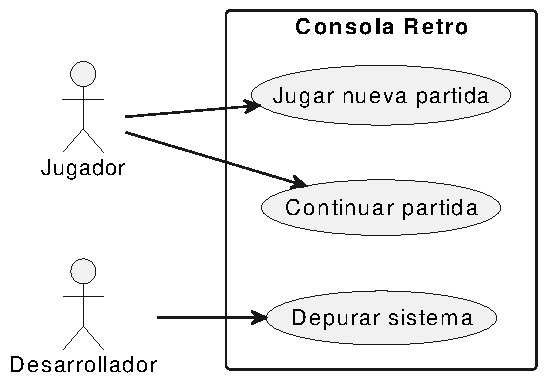
\includegraphics[width=.60\textwidth]{../Figuras/casos_uso.pdf}
% \caption{Diagrama de capas del sistema.}
\label{fig:diagCasosUso}
\end{figure}

% ────────── código PlantUML para generar la imágen en https://www.planttext.com/ ──────────
% @startuml
% left to right direction
% skinparam packageStyle rectangle
% actor Jugador
% actor Desarrollador

% package "Consola Retro" {
%   usecase "Jugar nueva partida"  as UC_Play_New
%   usecase "Continuar partida" as UC_Play_Old
%   usecase "Depurar sistema" as UC_Debug
% }

% Jugador       --> UC_Play_New
% Jugador       --> UC_Play_Old
% Desarrollador --> UC_Debug
% @enduml

\subsection{Caso de uso 1}
% ────────── CU-01 Jugar partida ──────────
\UseCaseTable
  {Jugar nueva partida} % #1 Nombre / título
  {El jugador inicia el sistema y juega hasta que decide salir, pudiendo guardar la partida o no.} % #2 Breve descripción
  {Jugador}             % #3 Actor principal
  {Encendido de la consola desde el switch de encendido.} % #4 Disparador
  {%
  \begin{enumerate}[leftmargin=*,nosep]
  \item El sistema muestra la pantalla de bienvenida.
  \item Luego de un tiempo máximo de 1,5 segundos, el sistema muestra el menú principal.
  \item El jugador selecciona la opción «Iniciar nueva partida».
  \item El sistema inicia el juego.
  \item El jugador juega el demo de simulación de vuelo.
  \item El jugador pausa el juego presionando el botón START en cualquier momento de la partida.
  \item El sistema muestra el menú de pausa con las opciones «Continuar», «Guardar» y «Salir».
  \item El jugador selecciona la opción «Guardar».
  \item El sistema muestra el mensaje «Guardado exitoso» y luego de un segundo muestra nuevamente el menú de pausa.
  \item El jugador selecciona la opción «Salir».
  \item El sistema sale del juego y retorna al menú principal.
  \item El jugador puede apagar la consola desde el switch de encendido.
  \end{enumerate}} % #5 Flujo básico
  {%
  \begin{enumerate}[leftmargin=*,nosep]
    \item Seguir jugando luego de la pausa.
  \begin{enumerate}[leftmargin=*,nosep]
    \item Desde el menú de pausa el jugador presiona la opción «Continuar».
    \item El juego retoma desde donde fué pausado.
  \end{enumerate}
    \item Guardado fallido.
    \begin{enumerate}[leftmargin=*,nosep]
      \item Al presionar la opción «Guardar» se muestra el mensaje «Error al guardar» y luego de un segundo se muestra nuevamente el menú de pausa.
    \end{enumerate}
  \end{enumerate}} % #6 Flujos alternativos
  {N/A} % #7 Requisitos especiales
  {Consola apagada.}    % #8 Pre-condiciones
  {Consola apagada.} % #9 Post-cond

\subsection{Caso de uso 2}
% ────────── CU-02 Continuar partida ──────────
\UseCaseTable
  {Continuar partida guardada} % #1 Nombre / título
  {El jugador retoma una partida previamente guardada.} % #2 Breve descripción
  {Jugador}             % #3 Actor principal
  {Encendido de la consola desde el switch de encendido.} % #4 Disparador
  {%
  \begin{enumerate}[leftmargin=*,nosep]
  \item El sistema muestra la pantalla de bienvenida.
  \item Luego de un tiempo máximo de 1,5 segundos, el sistema muestra el menú principal con las opciones «Iniciar nueva partida» y «Continuar».
  \item El jugador selecciona la opción «Continuar».
  \item El sistema inicia el juego cargando el estado de la partida guardada.
  \item El jugador continúa jugando su partida hasta que decide finalizar.
  \item El jugador pausa el juego presionando el botón START en cualquier momento de la partida.
  \item El sistema muestra el menú de pausa con las opciones «Continuar», «Guardar» y «Salir».
  \item El jugador selecciona la opción «Guardar».
  \item El sistema muestra el mensaje «Guardado exitoso» y luego de un segundo muestra nuevamente el menú de pausa.
  \item El jugador selecciona la opción «Salir».
  \item El sistema sale del juego y retorna al menú principal.
  \item El jugador puede apagar la consola desde el switch de encendido.
  \end{enumerate}} % #5 Flujo básico
  {%
  \begin{enumerate}[leftmargin=*,nosep]
    \item Seguir jugando luego de la pausa.
  \begin{enumerate}[leftmargin=*,nosep]
    \item Desde el menú de pausa el jugador presiona la opción «Continuar».
    \item El juego retoma desde donde fué pausado.
  \end{enumerate}
    \item Guardado fallido.
    \begin{enumerate}[leftmargin=*,nosep]
      \item Al presionar la opción «Guardar» se muestra el mensaje «Error al guardar» y luego de un segundo se muestra nuevamente el menú de pausa.
    \end{enumerate}
  \end{enumerate}} % #6 Flujos alternativos
  {Partida previamente guardada.} % #7 Requisitos especiales
  {Consola apagada.}    % #8 Pre-condiciones
  {Consola apagada.} % #9 Post-cond

\subsection{Caso de uso 3}
% ────────── CU-03 Debug ──────────
\UseCaseTable
  {Depurar el sistema} % #1 Nombre / título
  {El desarrollador habilita la salida de logs por la consola UART/USB, \
permitiendo observar el comportamiento interno del sistema en tiempo real.} % 1.1 Breve descripción
  {Desarrollador} % 1.2 Actor principal
  {El desarrollador envía el comando \texttt{logon} en la consola de depuración.} % 1.3 Disparador
  {% 2.1 Flujo básico
  \begin{enumerate}[leftmargin=*,nosep]
    \item La consola UART está disponible en cualquier estado del sistema.
    \item El desarrollador envía el comando \texttt{logon} por la consola.
    \item El sistema reconoce el comando, establece \texttt{logEnabled = true} y responde \texttt{LOG ON}.
    \item El sistema comienza a transmitir las trazas mientras \texttt{logEnabled} sea \texttt{true}.
    \item El desarrollador envía el comando \texttt{logoff}.
    \item El sistema reconoce el comando, establece \texttt{logEnabled = false} y responde \texttt{LOG OFF}.
    \item El sistema no envía trazas por la consola.
  \end{enumerate}}
  {% 2.2 Flujos alternativos
  \begin{enumerate}[leftmargin=*,nosep]
    \item \textit{Comando desconocido}: el sistema responde \texttt{ERR CMD} y mantiene el estado previo.
  \end{enumerate}}
  {La consola está conectada a 115\,200 bps con configuración 8N1.} % 3 Requisitos especiales
  {Al iniciar el sistema las trazas se encuentran deshabilitadas.} % 4 Pre-condiciones
  {N/A} % 5 Post-condiciones

\section{Apéndices}

N/A.

\end{document}
